\documentclass{beamer}



\usepackage{appendixnumberbeamer}
\usepackage{graphicx}
\usepackage{tikz}
\usepackage{booktabs}
\usepackage[scale=2]{ccicons}

\usepackage{pgfplots}
\usepgfplotslibrary{dateplot}

\usepackage{xspace}
\newcommand{\themename}{\textbf{\textsc{metropolis}}\xspace}

\usecolortheme{ibm}

\newcommand\ibmfooter{© 2020 IBM Corporation}
\usetheme[progressbar=frametitle]{metropolis}
\setbeamertemplate{frame numbering}[fraction]
\setbeamertemplate{frame footer}{\ibmfooter}
\useoutertheme{metropolis}
\useinnertheme{metropolis}
\usefonttheme{metropolis}
\title{IBM Cloud}
% \subtitle{Cloud Integration}
\author{Jaric Sng}
\institute{\textbf{IBM Cloud Integration (ASEAN)} \\ [2pt] Technology Architect \\ sngtpj@sg.ibm.com \\}
\titlegraphic{\includegraphics[scale=0.24]{../../img/icon.png}}
\date{}

\setbeamercolor{frame footer}{fg=blue90}
\usecolortheme[named=blue70]{structure}
\setbeamertemplate{frame footer}{\tiny{\ibmfooter{}}}
% \setbeamercolor{frame footer}{fg=white}
% \setbeamertemplate{frame footer}{\ibmfooter}

\begin{document}
% \metroset{titleformat frame=allcaps}	
\begin{frame}\vspace{10pt}
  \titlepage 
\end{frame}

\begin{frame}{Agenda}
  \setbeamertemplate{section in toc}[sections numbered]
  \tableofcontents%[hideallsubsections]
\end{frame}

\metroset{block=fill}
\section{Everything as Code}
\subsection{Examples}
\begin{frame}{Examples}
  \begin{columns}
    \begin{column}{0.5\textwidth}
      \begin{itemize}
        \item Infrastructure as Code\pause
        \item Configuration as Code\pause
        \item Securrity as Code\pause
        \item Workflow as Code\pause
        \item Architecture as code\pause
      \end{itemize}            
    \end{column}
    \begin{column}{0.5\textwidth}
      \begin{itemize}
        \item Document as Code\pause
        \item Presentation as Code\pause
        \item Training as Code \pause
        \item Diagram as Code \pause
        \item Operation as Code\pause
        \item Projects as code + Scaffolding 
      \end{itemize}            
    \end{column}
  \end{columns}
\end{frame}

\section{Values Proposition}
\begin{frame}{Values Proposition}
  \begin{columns}
    \begin{column}{0.5\textwidth}
      \begin{itemize}
        \item Reproducible\pause
        \item Tracebility\pause
        \item Identifiability\pause
        \item Clarity\pause
        \item Searchable\pause 
      \end{itemize}          
    \end{column}
    \begin{column}{0.5\textwidth}
      \begin{itemize}
        \item Reduced duplication\pause
        \item Reduced errors\pause
        \item Review\pause
        \item Collaboration\pause
        \item Scale
      \end{itemize}
    \end{column}
  \end{columns}
\end{frame}

\section{Version Control}
\begin{frame}{Benefits}
  \begin{itemize}
    \item Backup\pause
    \item Uppdate, Rollback\pause
    \item Identifies differences\pause
    \item Knowledge base\pause
    \item Collaboration\pause
    \item Accountability \pause
    \item Securrity - revision history
  \end{itemize}
\end{frame}

\section{Demo}

\begin{frame}{Diagram as Code - Draw}
  \begin{center}
    \begin{tikzpicture}
      \draw(0,0)rectangle(4,4);
    
      \draw(0,0)parabola (4,4);
      % \draw(0,0) .. controls(0,4) and (4,0) .. (4,4);        
  \end{tikzpicture}
  \end{center}
\end{frame}

\begin{frame}{Diagram as Code - Draw}
  \begin{center}
    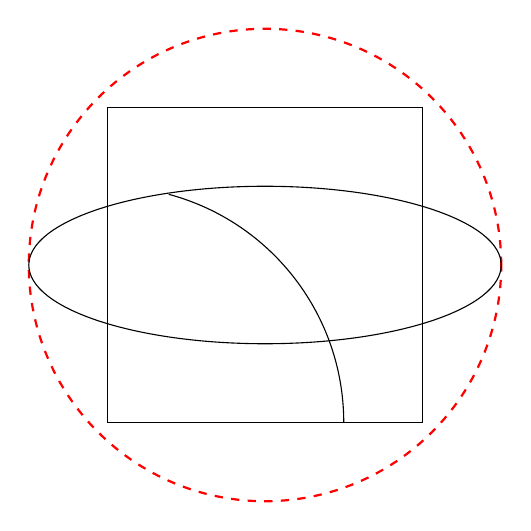
\begin{tikzpicture}
      \draw(0,0)rectangle(4,4);
      
      % \draw(0,0)parabola (4,4);
      % \draw(0,0) .. controls(0,4) and (4,0) .. (4,4);

      \draw[red,thick, dashed](2,2)circle(3cm);
      \draw(2,2)ellipse(3cm and 1cm);
      \draw(3,0) arc(0:75:3cm);
    \end{tikzpicture}
  \end{center}
\end{frame}

\begin{frame}{Diagram as Code - Draw}
  \begin{center}
    \begin{tikzpicture}
      \draw[step=1cm,gray,very thin](-2,-2)grid(5,5);
      % \filldraw[fill=blue!40!white, draw=black](0,0)rectangle(4,4);
      % \shade[left color=blue100,right color=blue10](0,0)rectangle(4,4);
      \shade[top color=blue100,bottom color=blue10](0,0)rectangle(4,4);
      % \shade[inner color=blue100,outer color=blue10](0,0)rectangle(4,4);
    \end{tikzpicture}
  \end{center}
\end{frame}

\begin{frame}{Diagram as Code - Graph}
  \begin{center}
    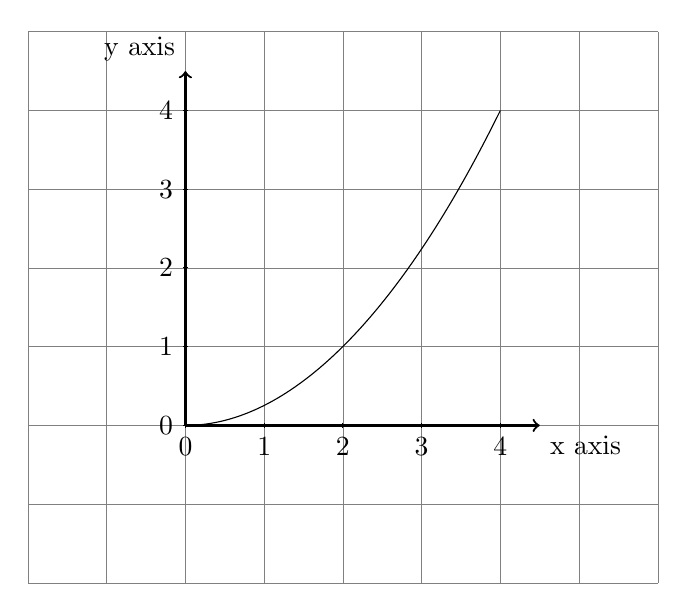
\begin{tikzpicture}
      \draw[step=1cm,gray,very thin](-2,-2)grid(6,5);
      \draw[thick,->] (0,0) -- (4.5,0)node[anchor=north west]{x axis};
      \draw[thick,->](0,0) --(0,4.5)node[anchor=south east]{y axis};
      \foreach \x in {0,1,2,3,4}
        \draw(\x cm,1pt)-- (\x cm,-1pt) node[anchor=north] {$\x$};
      \foreach \y in {0,1,2,3,4}
        \draw(1pt,\y cm)-- (-1pt,\y cm) node[anchor=east] {$\y$};

      \draw (0,0) parabola (4,4);
    \end{tikzpicture}
  \end{center}
\end{frame}

\begin{frame}[t]{Mathematic equation as Code}\vspace{10pt}
  \begin{block}{Definition of a Function}
    \vspace{0.5em}
    A \textbf{function} $f$ is a rule that assigns to each element $x$ in a set $D$ exactly one element, called $f(x)$, in a set $E$.
          \vspace{0.5em}
  \end{block}

\vspace{10pt}
Set $D$ is called the 
\only<1>{ \line(1,0){50} }
\only<2>{\textcolor{magenta}{domain}}
\, of the function. \\ [10pt]
Set $E$ is call the  
\only<1>{ \line(1,0){50} }
\only<2>{\textcolor{magenta}{range}}
\, of the function. 
\end{frame}

\begin{frame}[t]{Your Very First Flash Card}\vspace{10pt}
  \begin{columns}
    \column{0.5\textwidth}
    $\sqrt{x^2}=$\\[0pt]
    \begin{enumerate}[(a)]
      \item $x$
      \item $-x$
      \item $|x|$
      \item undefined
    \end{enumerate}  \vspace{40pt}
    \tiny{Online equation editor} 
    \href{https://latex.codecogs.com/legacy/eqneditor/editor.php}{\beamergotobutton{Link}}  
    \column{0.5\textwidth}\\[15pt]
    \begin{center}
      Plot for \\
      $ y = x^2, \sin x, \cos x, \tan x$
    \end{center}
    \includegraphics[scale=0.16]{../../img/graph.png}
  \end{columns}  
\end{frame}

\section{Conclusion}

\begin{frame}{Summary}

  Get the source from 

  \begin{center}
    \url{https://github.com/jaricsng/everything-as-code}
  \end{center}

  This is created based on Beamer Modern Metropolis Theme and can be obtained from 

  \begin{center}\url{github.com/matze/mtheme}\end{center}

  The theme \emph{itself} is licensed under a
  \href{http://creativecommons.org/licenses/by-sa/4.0/}{Creative Commons
  Attribution-ShareAlike 4.0 International License}.

  \begin{center}\ccbysa\end{center}

\end{frame}

{\setbeamercolor{palette primary}{fg=blue70, bg=white}
\begin{frame}[standout]
  Questions?
\end{frame}
}

{\setbeamercolor{palette primary}{fg=blue70, bg=white}
\begin{frame}[standout]
  Thank you
\end{frame}
}

% \section{Attribution}
\begin{frame}{Attribution}
  \begin{itemize}
    \item Michelle Krummel \LaTeX tutorial play list 
    \href{https://www.youtube.com/watch?v=0fsWGg81RwU&list=PL1D4EAB31D3EBC449&index=15}{\beamergotobutton{Link}}
    \item Matthias Vogelgesang \tiny\href{https://github.com/matze/mtheme}{\beamergotobutton{Link}}
  \end{itemize}    
\end{frame}

\begin{frame}[fragile]{Backup slides}
  Sometimes, it is useful to add slides at the end of your presentation to
  refer to during audience questions.

  The best way to do this is to include the \verb|appendixnumberbeamer|
  package in your preamble and call \verb|\appendix| before your backup slides.

  themename will automatically turn off slide numbering and progress bars for
  slides in the appendix.
\end{frame}

\end{document}